\setlength{\columnsep}{0.6cm}
% \setlength{\columnseprule}{1pt}
\chapter{Réalisation du pipeline}

%K4 <3

% TRACLUS ? présentation ?

\section{Compression de trajectoire}
\label{compression}

Pour permettre une analyse des données par les algorithmes en un temps raisonnable, la compression est une étape importante du traitement. Cependant, il y a un équilibre à trouver entre concision et précision. Pour y arriver, il a été décidé d'adopter le principe MDL (Minimum Description Length) et plus particulièrement, une méthode permettant de trouver une solution approximative en temps linéaire.

Nous nous basons ici sur le travail de \href{https://hanj.cs.illinois.edu/pdf/sigmod07_jglee.pdf}{Jae-Gil Lee et Kyu-Young Whang}~\cite{lee2007trajectory}. 

Pour réaliser cette compression, il faut introduire la notion de distance à choisir, quelles sont les propriétés désirables pour une compression de trajectoire, la formalisation à l'aide du principe MDL. Avant de terminer sur la solution approximative proposée. Cette méthode de compression rapide est nécessaire pour traiter de grandes quantités de données de trajectoires tout en préservant une précision suffisante pour l'analyse ultérieure.

\subsection{Propriétés désirables pour la compression de trajectoire}

L'objectif est de trouver des points caractéristiques tels qu'ils se trouvent à clés dans la représentation de la trajectoire, notamment lors de changements flagrants de direction. Avec l'idée d'un équilibre entre précision et concision. Comme illustré ci-dessous \ref{fig:mdlcost}.

\begin{figure}[ht]
    \centering
    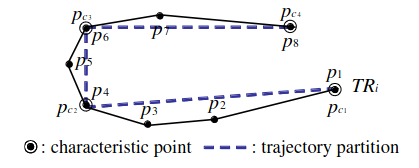
\includegraphics[width=0.5\textwidth]{Images/compressionExample.png}
    \caption{Exemple d'une trajectoire et de sa compression}
    \label{fig:mdlcost}
    Source : \href{https://hanj.cs.illinois.edu/pdf/sigmod07_jglee.pdf}{Trajectory Clustering: A Partition-and-Group Framework}
\end{figure}

\subsection{Fonction de distance}

Pour réaliser du clustering sur des segments de trajectoires, Jae-Gil Lee et Kyu-Young Whang ont défini une notion de distance composée de trois composantes comme suit : la distance perpendiculaire ($d_{\perp}$), la distance parallèle ($d_{\parallel}$) et la distance angulaire ($d_{\theta}$). Elles sont illustrées de manière intuitive dans la Figure~\ref{fig:distances}. Il est possible de voir le détail des calculs en annexe~\ref{an:compression_dist}.

Supposons que nous ayons 2 segments en $n$ dimensions, $L_i = s_i e_i$ et $L_j = s_j e_j$, où $s_i$, $e_i$, $s_j$ et $e_j$ représentent des points de $n$ dimensions. Nous assignons le segment plus long à $L_i$ et le segment plus court à $L_j$.


\begin{figure}[ht]
    \centering
    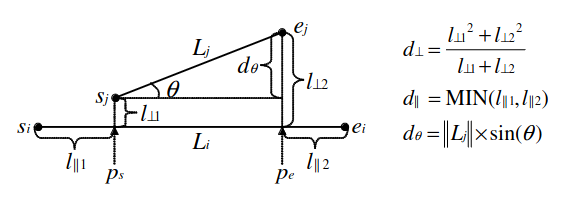
\includegraphics[width=0.44\textwidth]{Images/distances.png}
    \caption{Les 3 composantes de distance entre 2 segments}
    \label{fig:distances}
    Source : \href{https://hanj.cs.illinois.edu/pdf/sigmod07_jglee.pdf}{Trajectory Clustering: A Partition-and-Group Framework}
\end{figure}


\subsection{Principe MDL formalisé}

Le concept de Longueur de Description Minimum (MDL) est largement utilisé en théorie de l'information pour décrire un ensemble de théories et d'applications. L'idée clé de ce concept est que pour un ensemble de données (D) donné, la meilleure hypothèse (H) est celle qui conduit à la meilleure compression pour ces données. Les deux composantes de base de MDL sont : $L(H)$ et $L(D|H)$, où $L(H)$ est la longueur, en bits, de la description de l'hypothèse et $L(D|H)$ est la longueur, en bits, de la description des données lorsqu'elles sont encodées à l'aide de l'hypothèse. La meilleure hypothèse $H$ pour expliquer D est celle qui minimise la somme de $L(H)$ et $L(D|H)$. Ici, $L(H)$ mesure le degré de concision et $L(D|H)$ celui de l'exactitude.

\vspace{0.5cm}

En formalisant ce concept ici :
 \begin{equation}
    L(H) = \sum_{j=1}^{p-1} \log_2(\text{len}(pc_j pc_{j+1}))
\end{equation}

 \begin{equation}
    L(D|H) = \sum_{j=1}^{p-1} \sum_{k=c_j}^{c_{j+1}-1} {\log_2(d_\perp(pc_j pc_{j+1}, pk pk_{k+1})) + \log_2(d_\theta(pc_j pc_{j+1}, pk pk_{k+1}))}
\end{equation}

\begin{figure}[ht]
    \centering
    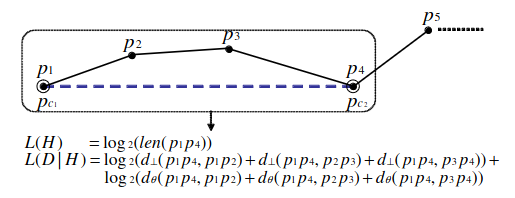
\includegraphics[width=0.6\textwidth]{Images/MDLcostExample.png}
    \caption{Exemple de la formalisation MDL sur un bout de trajecoires}
    \label{fig:mdlcost2}
    Source : \href{https://hanj.cs.illinois.edu/pdf/sigmod07_jglee.pdf}{Trajectory Clustering: A Partition-and-Group Framework}
\end{figure}


\subsection{Méthode de compression rapide en temps linéaire}

La méthode proposée consiste à considérer que l'ensemble des optima locaux est l'optimum global. Cela s'apparente à une observation de l'évolution de l'entropie locale, ici l'équilibre local entre le $L(H)$ et $L(D|H)$, en sélectionnant à chaque étape le point suivant comme point caractéristique. Si l'entropie augmente brusquement, il faut alors sélectionner le point précédent comme point caractéristique et reprendre à partir de celui-ci. Cela s'illustre bien sûr la figure \ref{fig:mdlcost}. Voir annexe pour plus de détails \ref{an:compression_lin}.



\section{Clustering}
\label{clustering}


Le clustering~\ref{fig_clustering} est une technique d'analyse de données qui permet de regrouper des données similaires ensemble en des groupes appelés "clusters". Le but du clustering est d'identifier des structures dans les données qui ne sont pas évidentes à observer à première vue.

Le clustering est une technique non supervisée, ce qui signifie qu'il n'y a pas de variable de réponse prédéfinie. Au lieu de cela, les algorithmes de clustering examinent les caractéristiques des données et les regroupent en fonction de leur similarité. Les données qui sont similaires sont regroupées dans le même cluster, tandis que les données qui sont différentes sont regroupées dans des clusters différents.

Il existe plusieurs types d'algorithmes de clustering, chacun avec ses propres avantages et inconvénients.
Le choix de l'algorithme de clustering dépendra des données et de l'objectif de l'analyse. Les clusters peuvent être utilisés pour découvrir des tendances ou des relations cachées dans les données, ou pour segmenter les clients en fonction de leurs caractéristiques communes.

\begin{figure}[!ht]
    \centering
    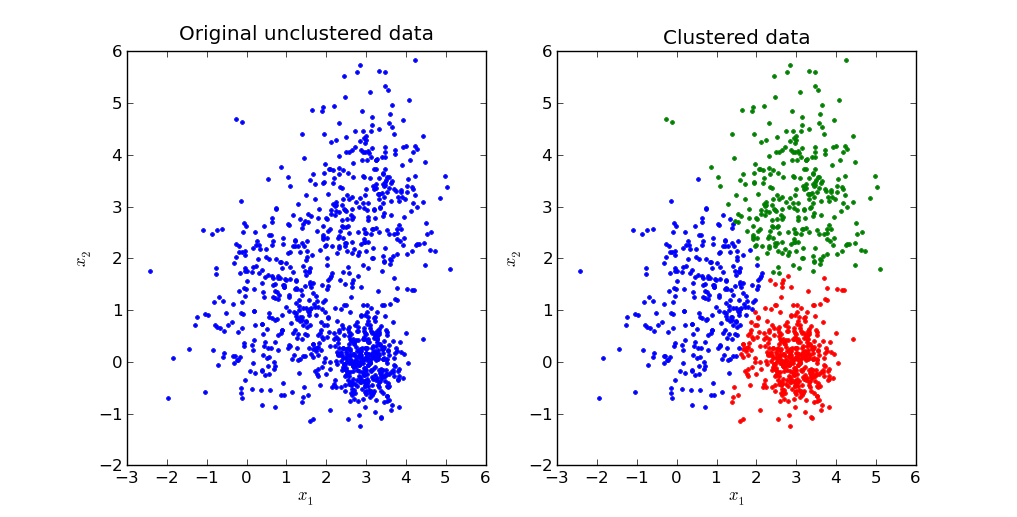
\includegraphics[width=1\textwidth]{Images/clustering.png}
    \caption{Exemple de clustering}
    \label{fig_clustering}
    Source : \href{https://mubaris.com/posts/kmeans-clustering/}{mubaris clustering}
\end{figure}

\newpage

\subsection{K-Means et K-Medoids}
\label{algo_k}
Fonctionnement de K-Means:

\begin{enumerate}
    \item spécifier le nombre de clusters(K).
    \item Ensuite, sélectionner K éléments de données initiaux qui serviront de centres de cluster. Ces éléments peuvent être choisis au hasard ou selon un critère spécifique.
    \item À présent, l'algorithme attribue chaque élément de données au cluster le plus proche en termes de distance. Cela signifie que chaque élément est assigné au centre de cluster le plus proche.
    \item Une fois que tous les éléments de données ont été attribués à un cluster, les centres de cluster sont recalculés en calculant la moyenne de tous les éléments qui leur ont été assignés.
    \item Les étapes 3 et 4 sont répétées jusqu'à ce que les centres de cluster ne changent plus, ou que le nombre d'itérations maximum soit atteint.
\end{enumerate}

À la fin du processus, chaque élément de données appartient à un cluster spécifique, et chaque cluster est caractérisé par son centre. L'algorithme K-means vise à minimiser la somme des distances entre chaque élément de données et son centre de cluster correspondant. C'est ce qu'on appelle la fonction objective de l'algorithme.

L'algorithme K-means est rapide et efficace pour de petits et moyens ensembles de données. Toutefois, il peut être sensible aux éléments de données initiaux sélectionnés au hasard, et il peut avoir du mal à trouver la solution optimale pour de grands ensembles de données ou pour des données ayant une structure complexe.

L'algorithme k-medoids est sensiblement similaire à celui de k-means. La différence étant qu'au lieu de prendre la moyenne du cluster comme centre, il faut prendre l'élément dont la somme des distances par rapport à tous les autres éléments du cluster est la plus petite. Cela permet de rester plus proche des données réelles. Mais cela représente un coût supplémentaire.

\subsection{Propagation d'affinité}
\label{propa}

La propagation d'affinité est un algorithme de clustering proposé par Brendan J. Frey et Delbert Dueck, basé sur des données qui utilise une approche de propagation de similarité entre les points de données pour former des clusters. L'algorithme de propagation d'affinité utilise donc des mesures de similarité entre les points de données pour déterminer les clusters. L'implémentation est décrite en détail dans l'annexe \ref{an:propa}.

\begin{enumerate}

    \item \underline{Initialisation}: initialiser quatre matrices, une pour la similarité, une pour les responsabilités, une pour les disponibilités et une matrice finale qui va nous permettre d'extraire les différents clusters. Ces matrices sont de taille N*N avec N, la taille de l'ensemble d'éléments.
    
    \item \underline{Calcul de la similarité}: calculer la similarité entre chaque paire d'élément de données en utilisant une mesure de similarité, pour ensuite remplir la matrice de similarité. Dans notre cas, nos éléments sont dotés d'une méthode afin de quantifier la distance d'un élément à un autre. L'intérêt de cette matrice est de quantifier à quel degré un élément est semblable à un autre.
    
    \item \underline{Calcul des responsabilités}: l'algorithme utilise ensuite les valeurs de la similarité pour calculer les responsabilités de chaque élément en tenant compte des valeurs de leur disponibilité. Les responsabilités mesurent l'importance d'un élément pour les autres points de données.\\ 
    \begin{figure}[ht]
        \centering
        \begin{equation}
            \begin{aligned}
                R\left ( i,k \right )\leftarrow S\left ( i,k \right ) - max\left \{ D\left ( i,k' \right ) + S\left ( i,k' \right ) \right \}\\
                k'\neq k\\
            \end{aligned}
        \end{equation}
        \caption{Formule de la responsabilité}
        \label{fig:responsibility}
    \end{figure}

    \item \underline{Calcul des disponibilités}: l'algorithme va ensuite utiliser la matrice des responsabilités pour mettre à jour la matrice des disponibilités. Les disponibilités mesurent l'importance des autres points de données pour un élément donné.
    \begin{figure}[ht]
        \centering
        \begin{equation}
            \begin{aligned}
                D\left ( i,k \right )\leftarrow min\left \{ O,R\left ( k,k \right ) + \sum max\left \{ 0,R\left ( i',k \right ) \right \} \right \}\\
                i' \neq i, i' \neq j\\
            \end{aligned}
        \end{equation}
        \caption{Formule de la disponibilité}
        \label{fig:avariability}
    \end{figure}

    \item \underline{Assignation des clusters}: les étapes 3 et 4 vont être réitérées un nombre n de fois dans notre implémentation. Notre algorithme va ensuite venir mettre à jour la matrice finale, souvent appelée matrice de "critère" ou de "préférence", elle assigne chaque élément à un cluster en fonction de la responsabilité maximale de chaque élément. Cette matrice se calcule en faisant le somme matricielle de de responsabilité et de la disponibilité.
    
\end{enumerate}

% \subsubsection{Comment avons-nous implémenté cet algorithme ?}
% Par soucis de lisibilité, notons :


% \begin{itemize}
%     \item S, la matrice de similarité.
%     \item R, la matrice de responsabilité.
%     \item D, la matrice de disponibilité.
% \end{itemize}
% % \begin{multicols}{2}
%     \hspace*{13px} La structure de nos matrices est faite pour pouvoir comparer un élément d'index I à un élément d'index J, il est donc nécessaire d'utiliser une structure de liste ordonnée et fixe.\\
%     Pour commencer, il nous faut remplir la matrice de similarité.
%     Chacun de nos objets donnés est capable au préalable de se comparer à d'autres objets du même type.\\
%     Une méthode distance nous permet donc de comparer un objet I à un objet J. \\ 
%     (Voir l'algorithme implémenté \ref{sec:simcalc})\\
%     % \begin{algorithmic}[1]
%     %     % \State $\texttt{Méthode de calcul de la similarité$
%     %     \State $E \gets \texttt{L'ensemble d'éléments}$
%     %     \State $T \gets \texttt{la taille de E}$
%     %     \State $S \gets \texttt{Une matrice de taille T*T}$
%     %     \For{\texttt{I allant de 0 à T}}
%     %         \For{\texttt{J allant de 0 à T}}
%     %             \State $S(I,J) \gets \texttt{E(I).distance(E(J))}$
%     %         \EndFor
%     %     \EndFor
%     % \end{algorithmic}
% % \end{multicols}

% % \begin{multicols}{2}
%     Mettre à jour la matrice de responsabilité se fait une fois la similarité calculée. (voir figure \ref{fig:responsibility})\\
%     De manière plus explicite, la responsabilité d'un élément i par rapport à k se calcule par sa valeur de similarité, moins la valeur maximale de la disponibilité pour les éléments i en considérant tous les autres points de données j, sauf l'élément k. De cette manière, nous pouvons quantifier l'importance d'un élément pour les autres éléments.\\
%     (Voir l'algorithme implémenté \ref{sec:rescalc})\\
%     % \begin{algorithmic}[1]
%     %     % \State $\texttt{Méthode de calcul de la responsabilité$
%     %     \State $E \gets \texttt{L'ensemble d'éléments}$
%     %     \State $T \gets \texttt{la taille de E}$
%     %     \State $S \gets \texttt{Une matrice de taille T*T}$
%     %     \For{\texttt{I allant de 0 à T}}
%     %         \For{\texttt{J allant de 0 à T}}
%     %             \State $V = \texttt{S[i] + D[i]}$
%     %             \State $V[i] = -\infty$ 
%     %             \State $V[k] = -\infty$
%     %             \State $R[i,k] = R[i,k] + (S[i,k] - max(v))$
%     %         \EndFor
%     %     \EndFor
%     % \end{algorithmic}
    
%     \hspace*{13px} Un paramètre que nous avons nommé "damping" est un paramètre d'amortissement compris entre 0 et 1 qui contrôle la quantité de propagation d'affinité entre les éléments. Nous l'appliquons à la formule de cette manière :\\ 
%     \begin{equation}
%         \begin{aligned}
%             R\left ( i,k \right ) = R\left ( i,k \right ) * damping + S\left ( i,k \right ) - (1 - damping) * max\left \{ D\left ( i,k' \right ) + S\left ( i,k' \right ) \right \}
%         \end{aligned}
%     \end{equation}\\
%     Plus ce paramètre tend vers 0, plus les éléments similaires ne seront regroupés qu'avec leurs voisins directs. Au contraire, plus le damping est proche de 1, plus les points de données similaires seront regroupés ensemble, indépendamment de leur position dans l'ensemble des éléments.\\
    
%     Mettre à jour la matrice de disponibilité se fait une fois la responsabilité mise à jour. \\ 
%     (Voir l'algorithme implémenté \ref{sec:avacalc})\\
%     % \begin{algorithmic}[1]
%     %     \State $E \gets \texttt{L'ensemble d'éléments}$
%     %     \State $T \gets \texttt{la taille de E}$
%     %     \State $R \gets \texttt{Une matrice de taille T*T}$
%     %     \For{\texttt{I allant de 0 à T}}
%     %         \For{\texttt{J allant de 0 à T}}
%     %             \State $V \gets \texttt{prendre colone k dans R}$
%     %             \If{$i\neq k$} 
%     %                 \State $V[i] = -\infty$ 
%     %                 \State $V[k] = -\infty$
%     %                 \State $V[V < 0] = 0$
%     %                 \State $D[i,k] = D[i,k] + min(0, R[k,k] + somme(V))$
%     %             \Else
%     %                 \State $V[k] = -\infty$
%     %                 \State $V[V < 0] = 0$
%     %                 \State $D[k,k] = D[k,k] + somme(V)$
%     %             \EndIf
%     %         \EndFor
%     %     \EndFor
%     % \end{algorithmic}
%     R(k,k) est l'élément de la matrice de responsabilité R correspondant à la similarité entre le point k et lui-même. La somme est prise sur tous les points de données i' autres que i et j, et mesure l'influence des autres points de données sur la disponibilité du point i pour être affecté au 
%     cluster contenant le point j. La fonction max est utilisée ici pour ne prendre en compte que les valeurs positives de la matrice de responsabilité, ne considérant donc que les éléments i' qui ont une similarité positive avec le point k. Enfin, la fonction min est là pour contraindre le résultat final à être négatif ou nul. Cela permet de quantifier l'importance des autres éléments pour un élément donné.\\
%     \hspace*{13px} Une fois le processus de mise à jour de la responsabilité et la disponibilité répété un certain nombre de fois, nous finissons par faire l'addition matricielle de la matrice de responsabilité avec celle de disponibilité pour pouvoir en extraire les clusters et leur représentant, nous appelons cette matrice la matrice de critère. La valeur de critère la plus élevée de chaque colonne est désignée comme exemplaire et les colonnes qui partagent le même exemplaire se trouvent dans le même cluster.\\
%     \hspace*{13px} Le processus de mise à jour de la responsabilité et la disponibilité sont exécutés un nombre arbitrairement de fois dans notre implémentation. Cependant, cet algorithme converge relativement rapidement, calculer la matrice de critère à chaque itération permettrait de détecter une convergence et ainsi éviter de réaliser des itérations inutiles. \\

% \end{multicols}

% \begin{multicols}
    \subsubsection{Quels sont les inconvénients d'un tel algorithme ?}
    \hspace*{13px} L'inconvénient principal de cet algorithme est sa complexité quadratique O(n²). L'algorithme de propagation d'affinité nécessite une grande quantité de mémoire pour stocker ses matrices, qui sont des matrices carrées de la taille de l'ensemble au carré. Pour de grands ensembles de données, cela peut nécessiter une quantité considérable de mémoire, ce qui peut rendre l'exécution de l'algorithme difficile, voire impossible sur des ordinateurs avec une mémoire limitée.\\
    Le temps d'exécution est lui aussi impacté par la taille du jeu de donnée à traiter.
    
    \subsubsection{Quels en sont les avantages ?}
    
    \hspace*{13px} Bien que la complexité de cet algorithme puisse réduire le nombre d'applications de cet algorithme, son principal avantage est que contrairement aux méthodes de clustering traditionnelles, propagation d'affinité n'a pas besoin de connaitre le nombre de clusters à assigner, il va automatiquement le trouver tout en gardant une certaine pertinence des résultats.\\
    Malgré sa complexité, les calculs des matrices de cet algorithme sont parallélisables, rendant le calcul de celles-ci moins contraignantes sur de grands jeux de données.\\
    Une autre optimisation de cet algorithme est d'implémenter les itérations en calcul matriciel au lieu d'utiliser des boucles, rendant le calcul bien moins couteux en temps.
    
sources :\\
\href{https://utstat.toronto.edu/reid/sta414/frey-affinity.pdf}{Rapport de Brendan J. Frey et Delbert Dueck}\\
\href{https://github.com/scikit-learn/scikit-learn/blob/main/sklearn/cluster/_affinity_propagation.py}{Implémentation faite par la librairie  scikit-learn}\\
\href{https://towardsdatascience.com/unsupervised-machine-learning-affinity-propagation-algorithm-explained-d1fef85f22c8}{Publication de Towards Data Science}\\

%%%%%%%%%%%%%%%%%%%%%%%%%%%%%%%%%%%%%%%%%%%%%%%%%%%%
%\newpage

\section{Extraction de connaissance dans les données}
\label{extraction}

L'extraction de connaissance est le processus d'extraction d'informations utiles et exploitables à partir de sources de données brutes et non structurées, telles que des documents, des bases de données, des fichiers texte, des images, des vidéos et d'autres types de médias numériques.\\
Les principales taches de l'extraction des données sont le \textbf{clustering}, l'analyse des valeurs \textbf{aberrantes}, la \textbf{classification} et l'\textbf{extraction de motif fréquents}.
\subsection{Extraction séquentielle}
L'extraction séquentielle est une technique d'analyse de données qui consiste à identifier des motifs séquentiels récurrents dans une série temporelle ou une séquence d'événements.\\
Plus précisément, l'extraction séquentielle recherche des sous-séquences qui se produisent fréquemment dans une séquence donnée et les identifie comme des motifs significatifs. Ces motifs peuvent ensuite être utilisés pour comprendre le comportement de la séquence, pour prédire des événements futurs, pour détecter des anomalies ou pour d'autres applications.\\
Par exemple, si l'on analyse les achats d'un client sur une période, l'extraction séquentielle pourrait identifier des motifs tels que "le client achète toujours du café après avoir acheté du lait". Cela pourrait aider une entreprise à mieux comprendre les préférences du client et à proposer des offres ciblées.\\
En résumé, l'extraction séquentielle est une technique utile pour trouver des modèles récurrents dans une série temporelle ou une séquence d'événements, ce qui peut aider à mieux comprendre le comportement et à prendre des décisions éclairées en conséquence.
\subsubsection{Exemple}
\begin{figure}[ht!]
    \centering
    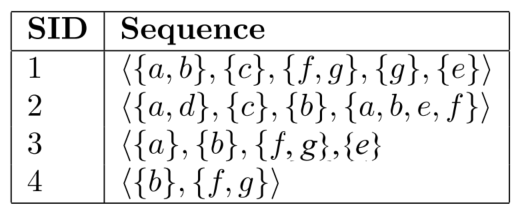
\includegraphics{Images/seq2-1.png}
    \caption{Exemple de séquence d'items}
    \label{fig:seq}
    source : \href{https://data-mining.philippe-fournier-viger.com/wp-content/uploads/2017/03/seq2-1.png}{The data mining blog}
\end{figure}
Dans cet exemple \ref{fig:seq}, les données en question contiennent quatre séquences de transactions d'achats effectuées par différents clients. Chaque séquence représente les articles achetés par un client à différents moments. Une séquence est une liste ordonnée d'ensembles d'articles achetés ensemble, appelés itemsets.\\
Dans cet exemple \ref{fig:seq}, la première séquence (identifiée par SID 1) indique que le client a acheté des articles a et b ensemble, puis a acheté l'article c seul, ensuite a acheté les articles f et g ensemble, puis a acheté l'article g seul, et enfin a acheté l'article e seul.\\
Dans cet exemple \ref{fig:seq}, nous pouvons noter que le pattern séquentiel $\langle$\{a\},\{f,g\}$\rangle$ qui apparait dans deux transactions une et deux, elle est donc un motif fréquent avec un support de 2, le support étant le nombre de transactions contenant cette séquence. De même, nous pouvons voir le pattern $\langle$\{a\},\{g\}$\rangle$ est un motif fréquent avec un support de 3, car apparaissant dans les transactions 1, 2 et 3.\\

Dans notre situation, nous cherchons donc des motifs fréquents qui illustreront les déplacements des joueurs lors des games. Par exemple, si le pattern $\langle$\{A\},\{F\},\{R\}$\rangle$ exprimant les positions du joueur est motif qui apparait de manière fréquente lors des games, il exprimera le fait que si le joueur se trouve (appartient) à un moment T au cluster A il ira ensuite au cluster F, puis B avec un certain  niveau de confiance, avec la confiance représentant la probabilité de réalisation.
